\section{Representative Examples}
\HHZ{I feel that the first example could serve as a demonstration that this downfolding approach works. Since both the original system and the downfolded model could be exactly solved, and are clean. It would be good if we could find some physical properties that both the two models produce the same values. The energy spectrum has been used as an input in the sense of "machine learning", it would be good if we could have a way to test the predicting power.}
\HJC{I agree, this was my motivation for spending the most time on it since it is a clean system. 
But this is at odds with shortening the section. Let me see if I have the 8 site results, that may build confidence in the results}

Given the theoretical framework for downfolding a many-orbital (or many electron) problem to a 
few orbital (or few electron) problem, we now discuss few examples which also serve to highlight some practical aspects 
associated with AIDMD. The first example is mostly pedagogical, 
where we have completely avoided the \emph{ab-initio} related complications of AIDMD. Rather, we use information directly available 
from \emph{exact} eigenstates themselves to downfold from a lattice model with more orbitals (3-band model) 
to one with fewer orbitals (1-band model). We then gradually increase the complexity of the problems we address
by downfolding the hydrogen chain in one dimension (with up to 10 atoms) and graphene 
(with up to 32 carbons on a 2D honeycomb lattice). 

A common occurrence in all our examples is the 1-band Hubbard Hamiltonian, defined as,
\begin{equation}
	\tilde{H} = -t \;\sum_{\langle i,j \rangle} \tilde{d}_i^{\dagger} \tilde{d}_j + U \;\sum_{i} \tilde{n}^{i}_{\uparrow} \tilde{n}^{i}_{\downarrow}
\label{eq:oneband}
\end{equation}
where $t$ and $U$ correspond to downfolded (renormalized) parameters and $\tilde{d}$ are the effective one-particle operators, 
which are obtained from transformations on their bare counterparts. This choice is crucial for obtaining accurate Hamiltonians 
and we highlight it for each example presented.   

\subsection{Three-band Hubbard model to one band Hubbard model at half filling}
\lucas{This section seems rather long to me. We should think about how to cut it down to the essentials.} 
\HJC{Working on it, but I think this section really clarifies downfolding, because it is a controlled setting. 
so making it too short is not a good idea. I agree we need to keep the essentials only.} 

Our first example is motivated by the high $T_c$ superconducting cuprates~\cite{Bednorz1986} that 
have parent Mott insulators with rich phase diagrams on electron or hole doping~\cite{Dagotto_RevModPhys, LeeWen_RevModPhys}. 
Many works have been devoted to their model effective Hamiltonians and corresponding parameter 
values~\cite{Emery, ZhangRice, tJSpalek, Hybertsen_PRB1989, Hybertsen_PRB1990, Pavirini, Kent_Hubbard}. 
The emergent consensus of the minimal model involving the oxygens is the 3-orbital or 3-band Hubbard model, 
\begin{eqnarray}
H &=&    \epsilon_p \sum_{j,\sigma} n^{p}_{j,\sigma} + \epsilon_{d} \sum_{i,\sigma}  n^{d}_{i,\sigma} 
	+ t_{pd} \sum_{\langle i,j \rangle, \sigma} \text{sgn}(p_i,d_j) \Big( d_{i,\sigma}^{\dagger} p_{j,\sigma} + \text{h.c.} \Big) \nonumber \\
  & &   + U_p \sum_{j} n^{p}_{j,\uparrow} n^{p}_{j,\downarrow} + U_d \sum_{i} n^{d}_{i,\uparrow} n^{d}_{i,\downarrow} + V_{pd} \sum_{\langle i,j \rangle} n^{j}_p n^{i}_d 
\end{eqnarray}
where $d_i,p_j$ refer to the  $d_{x^2 - y^2}$ orbitals of copper (at site $i$) and $p_x$ or $p_y$ 
oxygen (at site $j$)  respectively and the signs of the hopping $t_{pd}$ between them are shown in Fig.~\ref{fig:threeband}. 
$\epsilon_d$,$\epsilon_p$ refer to the orbital energies, 
$U_d$, $U_p$ refer to strength of onsite Hubbard interactions and $V_{pd}$ refers to the 
strength of the density-density interactions between a neighboring $p$ and $d$ orbital. 
We keep the exposition simple and consider only the case where $\epsilon_p$, $t_{pd}$ and $U_{d}$ are non zero
(since we work with fixed number of particles we set $\epsilon_d = 0$). 
The charge transfer energy $\Delta \equiv \epsilon_p - \epsilon_d$ equals $\epsilon_p$ in our notation. 
We work in the hole notation; half filling corresponds to 2$\uparrow$ and 2$\downarrow$ 
holes on the $2\times2$ cell.

\begin{figure}[htpb]
\centering
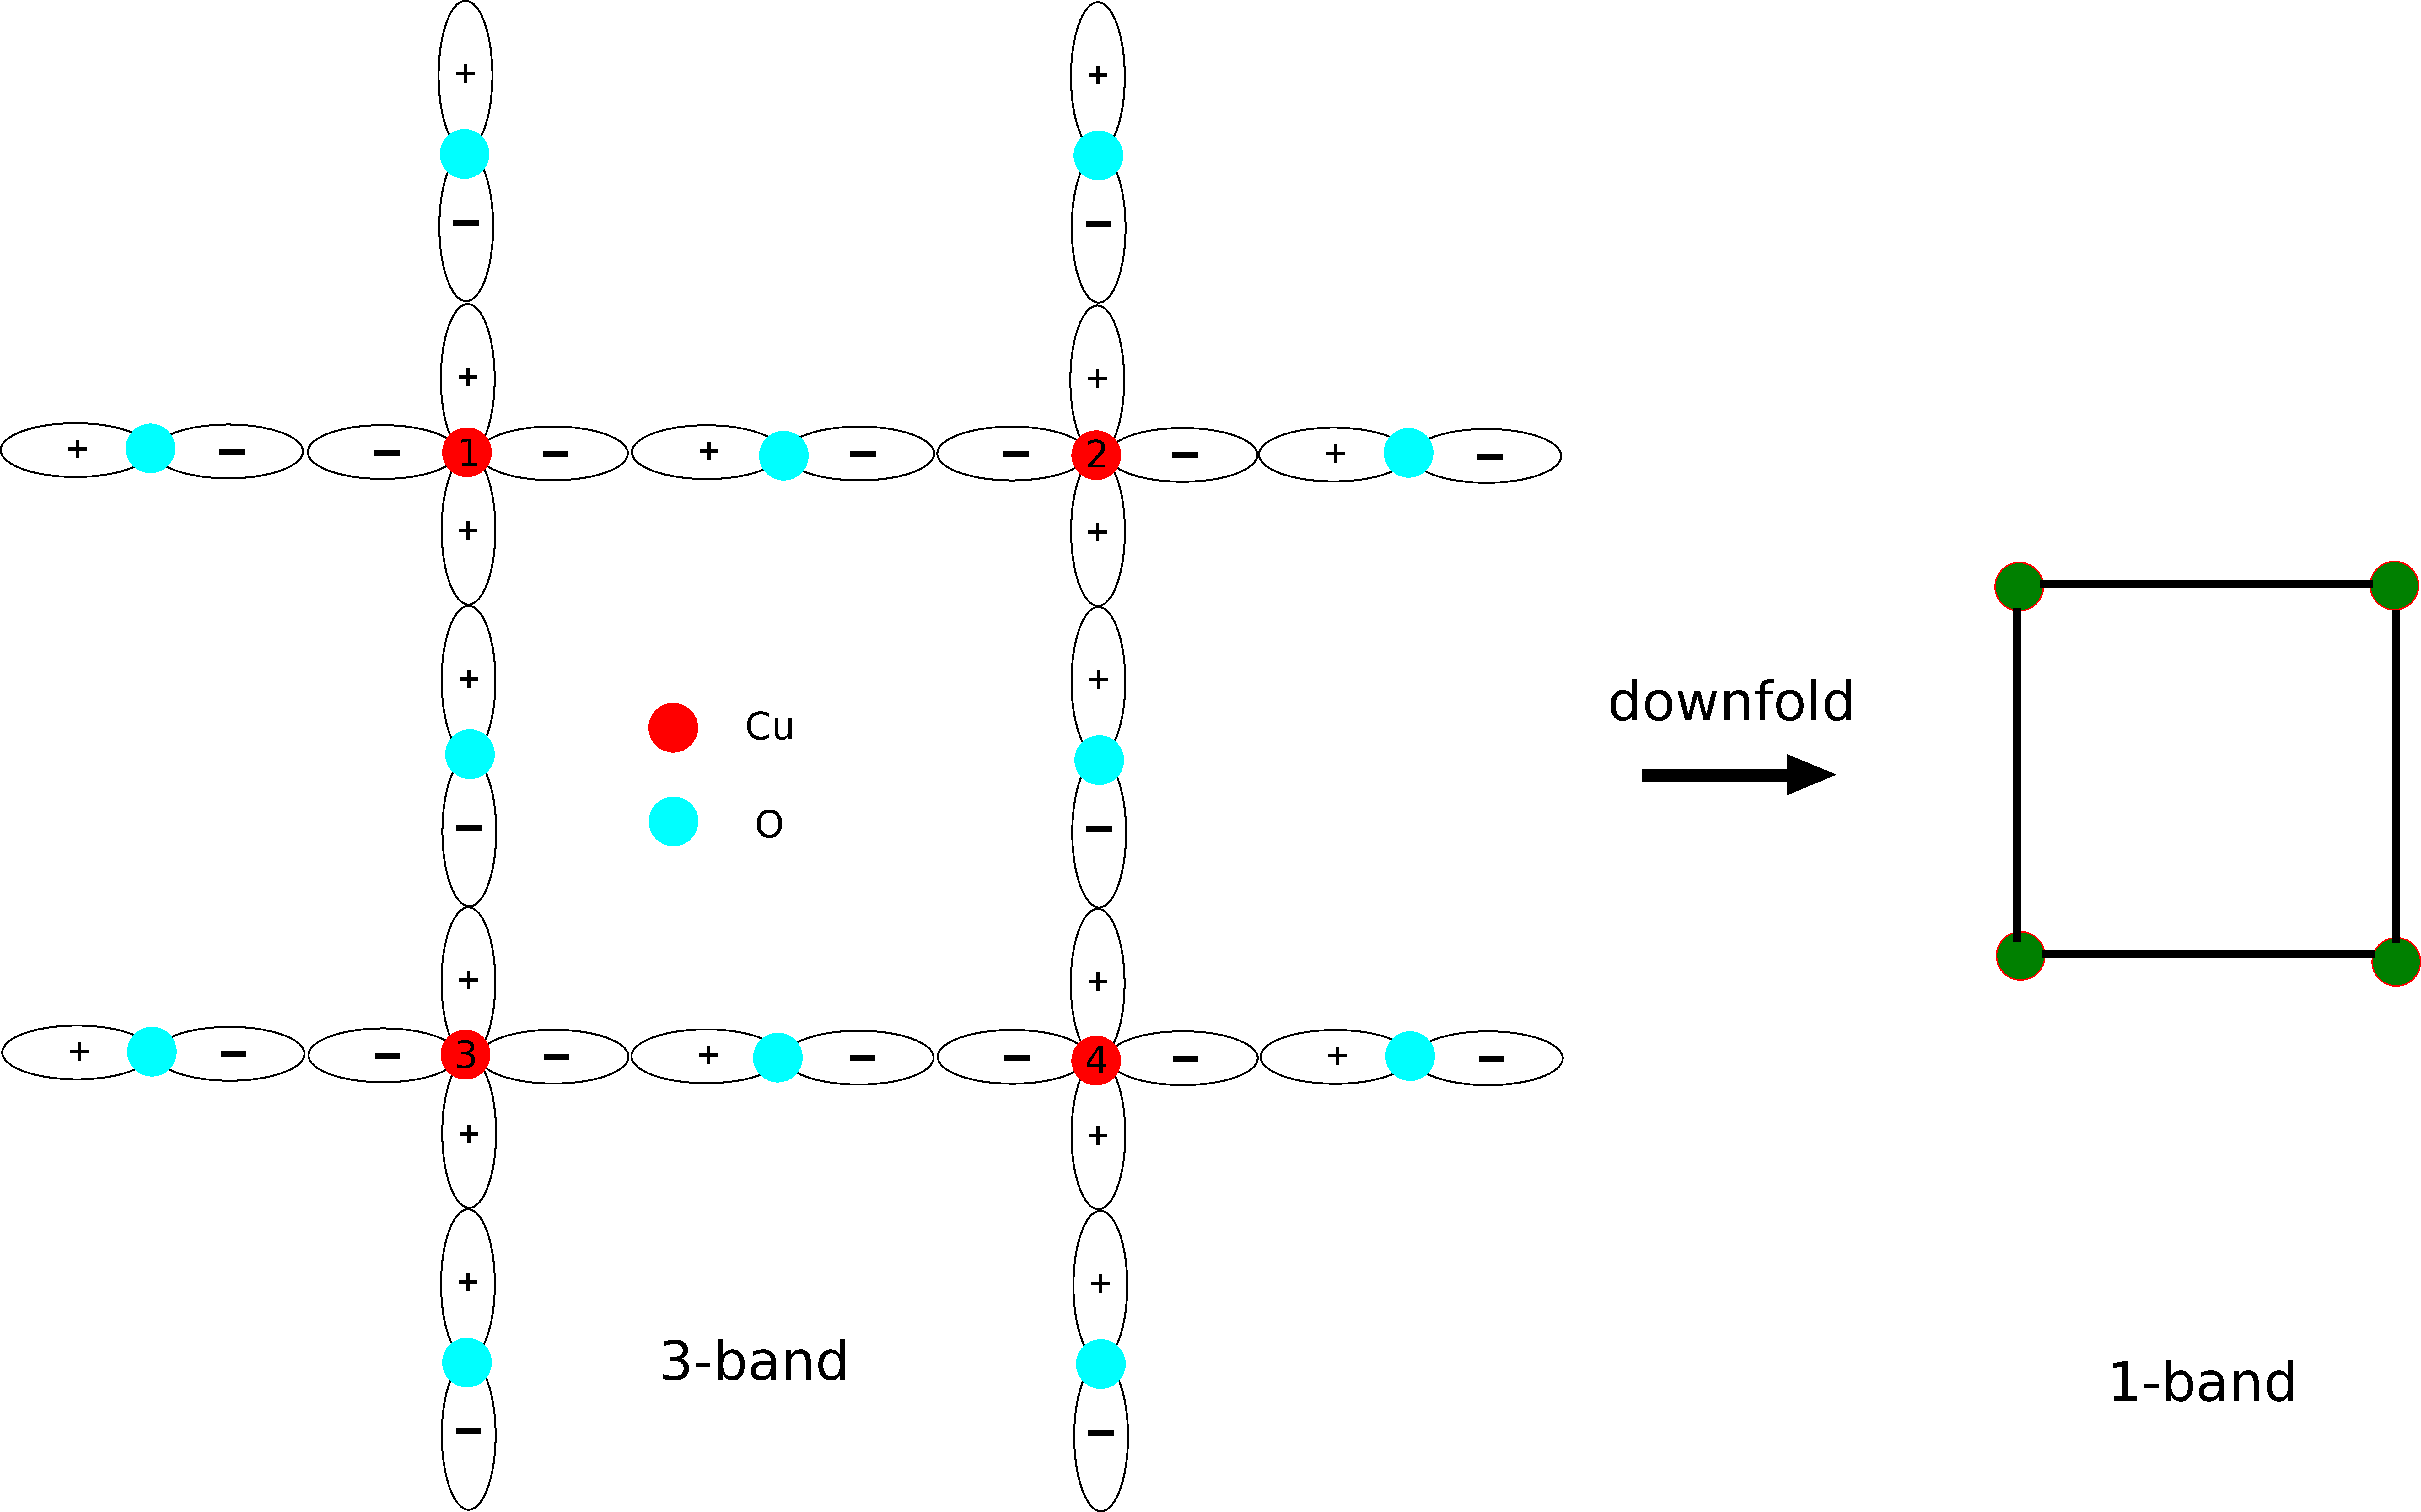
\includegraphics[width=0.8\linewidth]{./Figures/three_band_figure.pdf}
\caption{Schematic for downfolding the three band Hubbard model to the one band Hubbard model. 
The oxygen orbitals are completely eliminated to give "dressed" $d$-like orbitals of the one band model, with modified hopping 
and interaction parameters.}
\label{fig:threeband} 
\end{figure}	

We determine here, what 1-band parameters best describe the 3-band data, the former defined 
in terms of effective \emph{d-like} orbitals, $\tilde{d}$, which are mixtures of copper and oxygen orbitals. 
This optimal transformation also remains an unknown; we encode the relationship between the 
bare and effective operators as a linear transformation ${\bf T}$, 
\begin{equation}
	\tilde{d}_i = \sum_{j} T_{ij} c_j
\end{equation}
%where $\tilde{d}_i$ is a transformed hole (destruction) operator 
where $c_j$ is the bare hole (destruction) operator and refers to either the bare $d$ or $p$ orbitals. 
(Note that higher body generalizations are also possible, but have not been consisdered here). 
Accounting for all symmetries of the $2\times2$ unit cell, {\bf T} is a $4 \times 12 $ matrix (the numbering of the orbitals 
corresponds to Fig.~\ref{fig:threeband}) is explicitly written out as, 
\begin{eqnarray}
{\bf T} = 
\left(
\begin{array}{cccccccccccc}
F        & \alpha_2 &        \alpha_2 &  \alpha_4 & \alpha_1 & \alpha_1 & -\alpha_1 & -\alpha_1 & \alpha_3 & -\alpha_3 & \alpha_3 & -\alpha_3 \\
\alpha_2 &  F       &        \alpha_4 &  \alpha_2 & \alpha_3 & -\alpha_1 & \alpha_1 & -\alpha_3 & -\alpha_3 & \alpha_3 & \alpha_1 & -\alpha_1 \\
\alpha_2 & \alpha_4 & F               &  \alpha_2 & -\alpha_1 & \alpha_3 & -\alpha_3 & \alpha_1 & \alpha_1 & -\alpha_1 & -\alpha_3 & \alpha_3 \\
\alpha_4 & \alpha_2 & \alpha_2        &   F       & -\alpha_3 & -\alpha_3 & \alpha_3 & \alpha_3 & -\alpha_1 & \alpha_1 & -\alpha_1 & \alpha_1 \\
\end{array}
\right)
\end{eqnarray}
where we have defined $F \equiv \sqrt{1-4{\alpha_1}^2 - 2{\alpha_2}^2 - 4 {\alpha_3}^2 -{\alpha_4}^2}$ and 
where the parameters $\alpha_1$,$\alpha_2$,$\alpha_3$ and $\alpha_4$ will be optimized to minimize a 
certain cost function, which will be explained shortly. 

The one particle density matrix in the transformed basis is related 
to that in the original basis by,
\begin{equation}
	\langle {\tilde{d}_i}^{\dagger} \tilde{d}_{j} \rangle = \sum_{mn} T^{*}_{im} \langle {c_m}^{\dagger} c_n \rangle T_{jn}
\end{equation}
and using this relationship we demand two conditions be satisfied,
\begin{itemize} 
 \item The effective orbitals are orthogonal to each other 
 \item All diagonal entries of the 1-RDM of the effective orbitals for all low energy eigenstates 
       $(\langle {\tilde{d}_i}^{\dagger} \tilde{d}_{i} \rangle)$ 
       equal 1/2.
\end{itemize} 
We consider a cost function, 

To give a concrete and representative example of our results, we start with 1-RDM of the lowest eigenstate 
in either $\uparrow$ or $\downarrow$ channel. This is a $12 \times 12$ matrix, which for $U_{d}/t_{pd}=8$ 
and $\Delta/t_{pd}=3$ we find to be,
corresponding to the optimal parameters $\alpha_1=0.220$,$\alpha_2=0.044$,$\alpha_3=0.020$ and $\alpha_4=0.018$ 
We then ask what $U/t$ of the one band Hubbard model best describes this 1-RDM and in this case find $U/t = $. 
Similar results are found when one considers the other low energy eigenstates. 
(In practice, we minimize the sum of costs of the lowest three eigenstates on the $2 \times 2$ cluster.) 

\begin{figure}[]
\centering
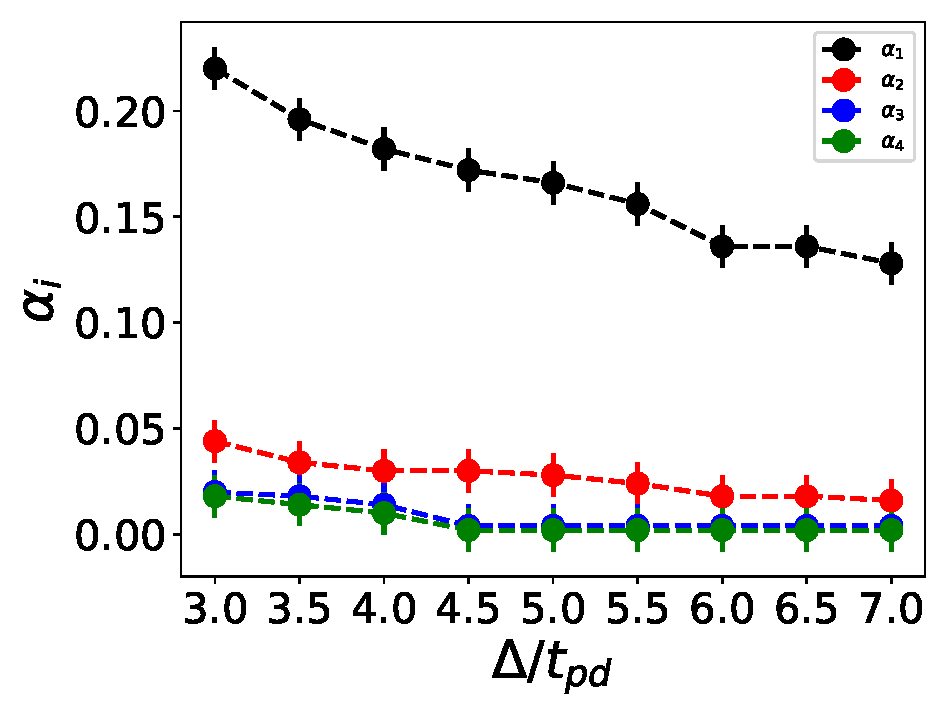
\includegraphics[width=0.32\linewidth]{./Figures/Hyb_vs_U_Ud_8.pdf}
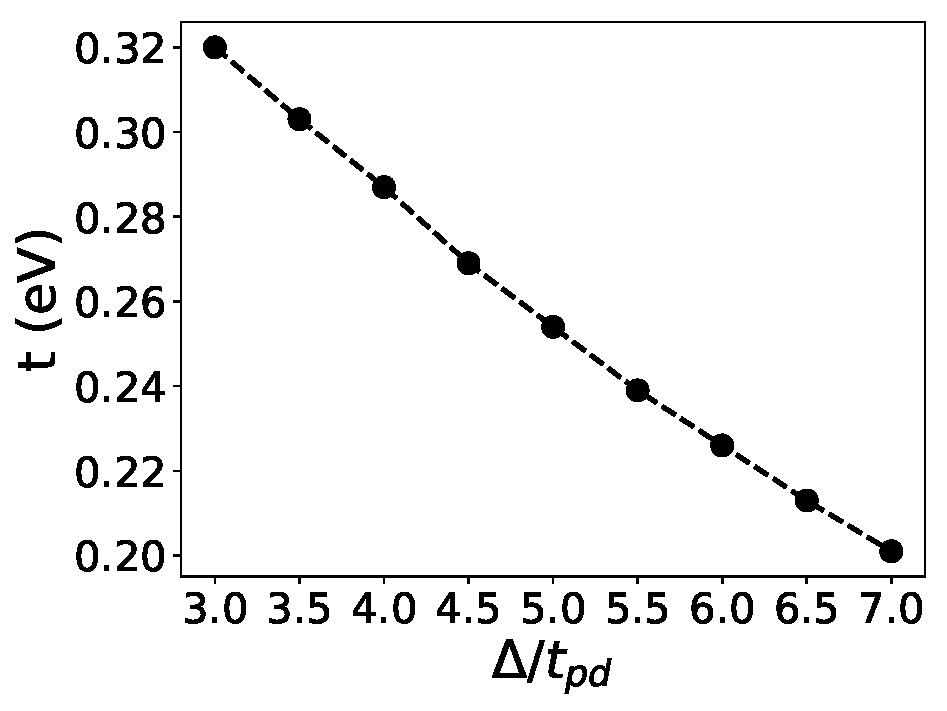
\includegraphics[width=0.32\linewidth]{./Figures/Hopping_vs_U_Ud_8.pdf}
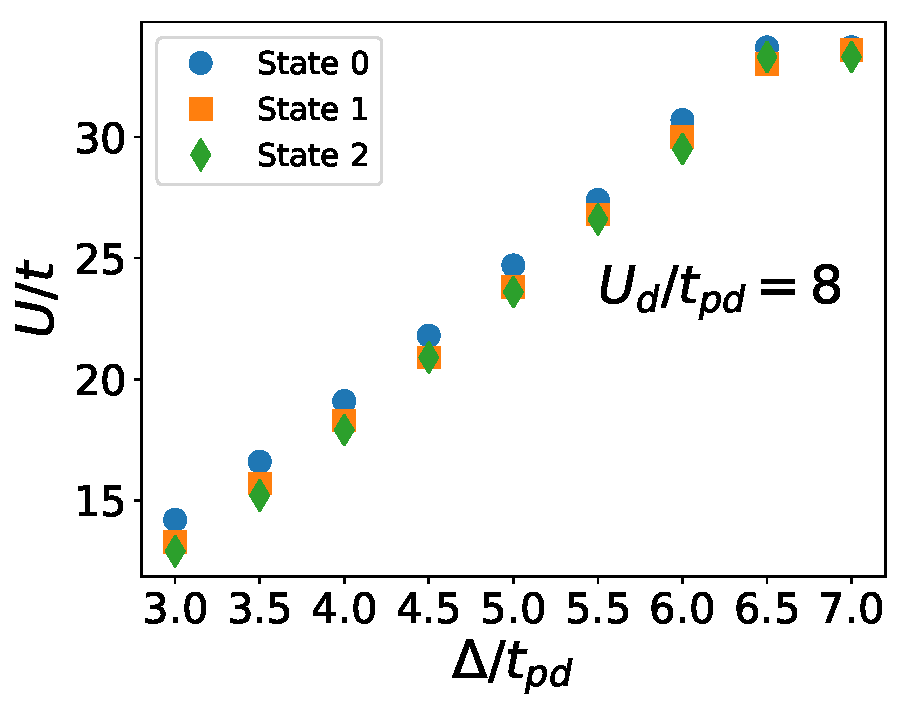
\includegraphics[width=0.32\linewidth]{./Figures/downfolded_U_Ud_8.pdf}
\caption{Downfolded values of the effective 1-band Hubbard U/t and hopping $t_{opt}$ vs $U_d/t_{pd}$}
\label{fig:hamfit} 
\end{figure}	

\begin{figure}[]
\centering
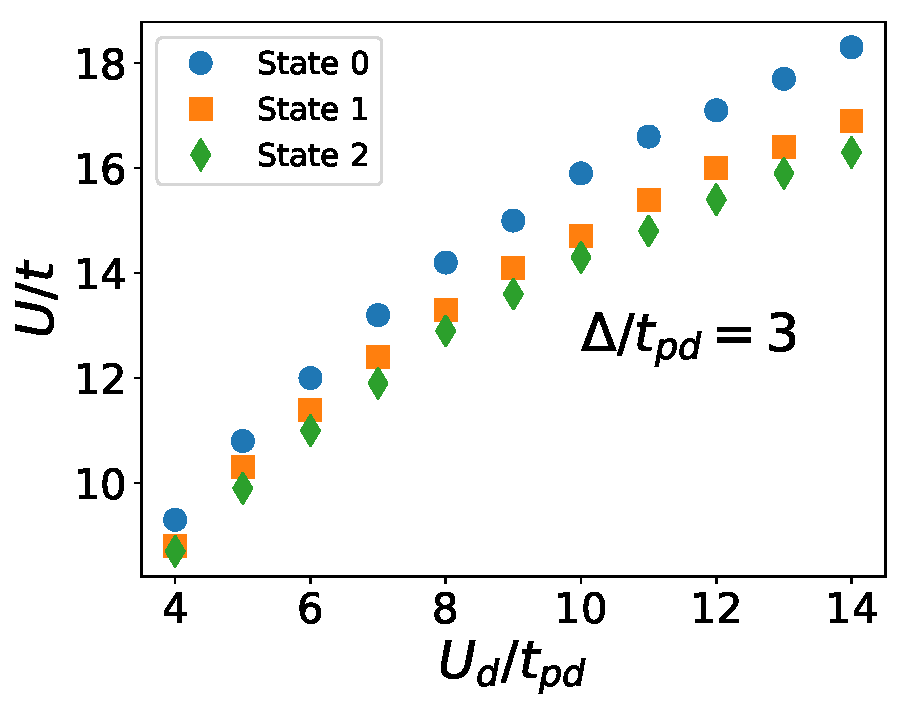
\includegraphics[width=0.49\linewidth]{./Figures/downfolded_U_ep_3.pdf}
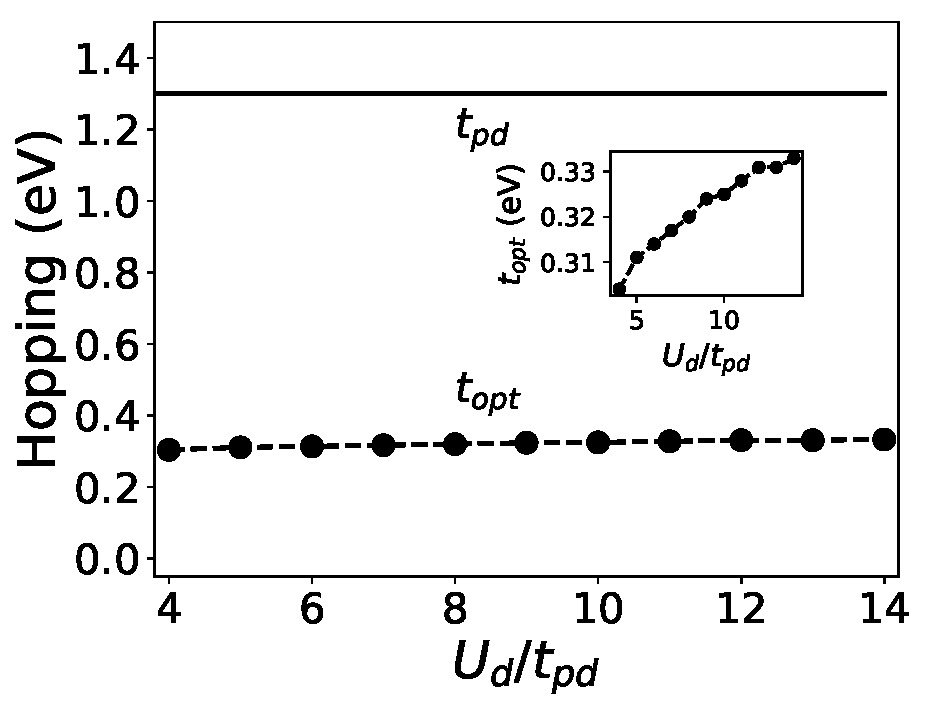
\includegraphics[width=0.49\linewidth]{./Figures/Hopping_vs_U_ep_3.pdf}
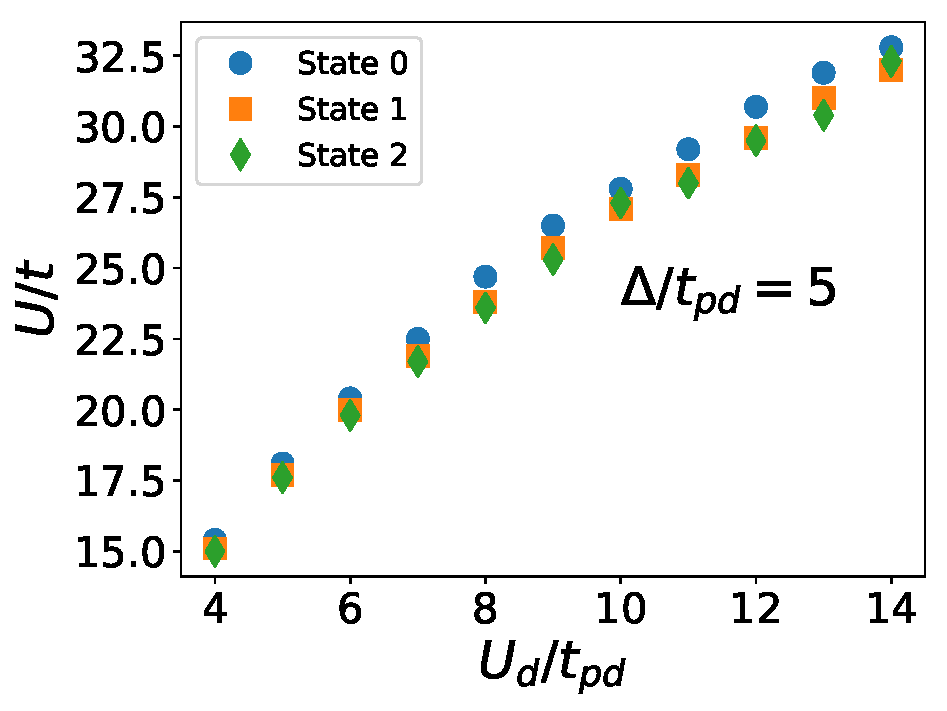
\includegraphics[width=0.49\linewidth]{./Figures/downfolded_U_ep_5.pdf}
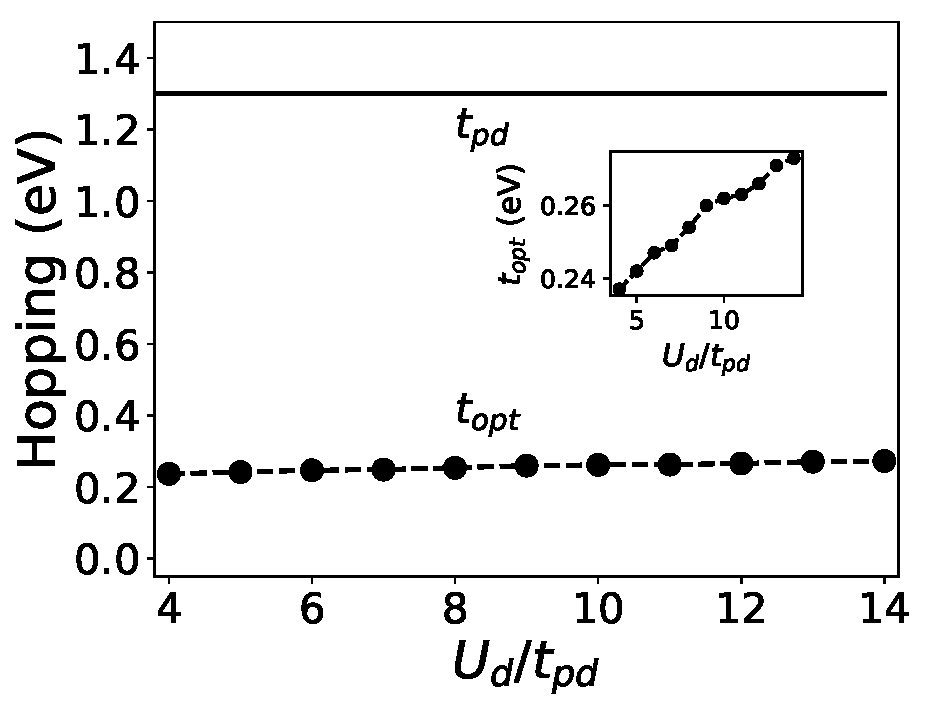
\includegraphics[width=0.49\linewidth]{./Figures/Hopping_vs_U_ep_5.pdf}
\caption{Downfolded values of the effective 1-band Hubbard U/t and hopping $t_{opt}$ vs $U_d/t_{pd}$}
\label{fig:hamfit} 
\end{figure}	
 
The density matrix matching does not provide an absolute energy scale for the matching. 
Taking $t_{pd}$ to be the typical values of $1.3$ eV, we then 
We show our results for the optimal values of $t$ and the transformation parameters for different $\Delta/t_{pd}$
keeping $U_d/t_{pd}=8$ fixed. First, note that $\alpha_1$, which is the primary parameter that mixes (hybridizes) 
the copper and oxygen orbitals, \emph{decreases} as $\Delta/t_{pd}$ is increased. This is physically reasonable 
since an increasing difference in the single particle energies of the copper and oxygen orbitals 
means that it is even more energetically unfavorable to occupy the oxygen orbitals. 
Correspondingly the effective hopping between $\tilde{d}$ in the 
1-band model reduces and the effective $U/t$ increases. 

Next, we consider our results for  

These results are only useful if the energy spectra between the two models also matches. This is verified 
and demonstrated for some representative examples in Fig.        

\begin{figure}[]
\centering
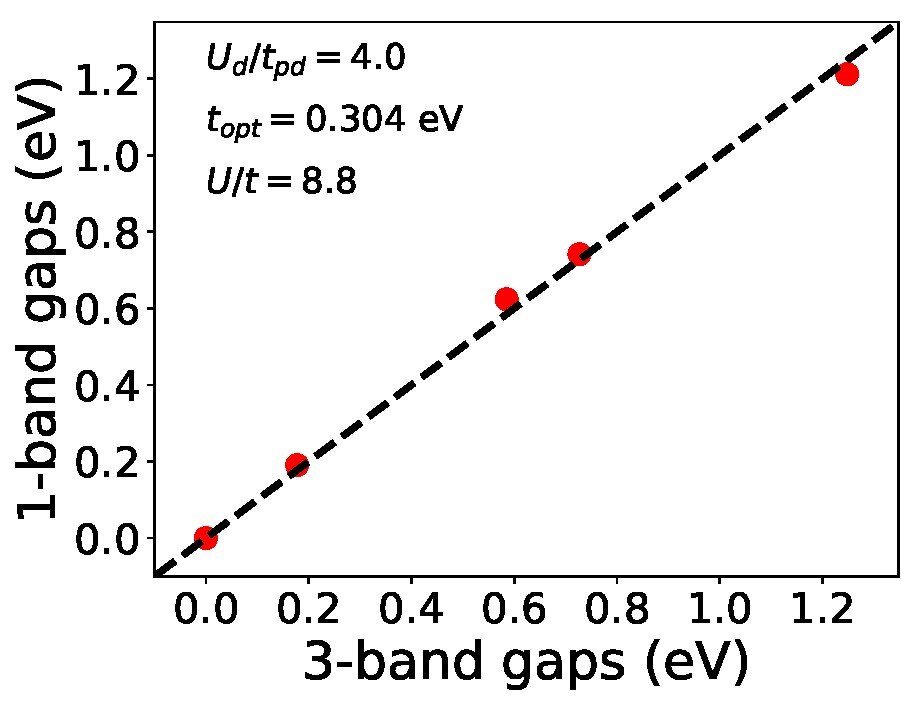
\includegraphics[width=0.325\linewidth]{./Figures/Gap_1_band_3_band_ep_3_number_5.pdf}
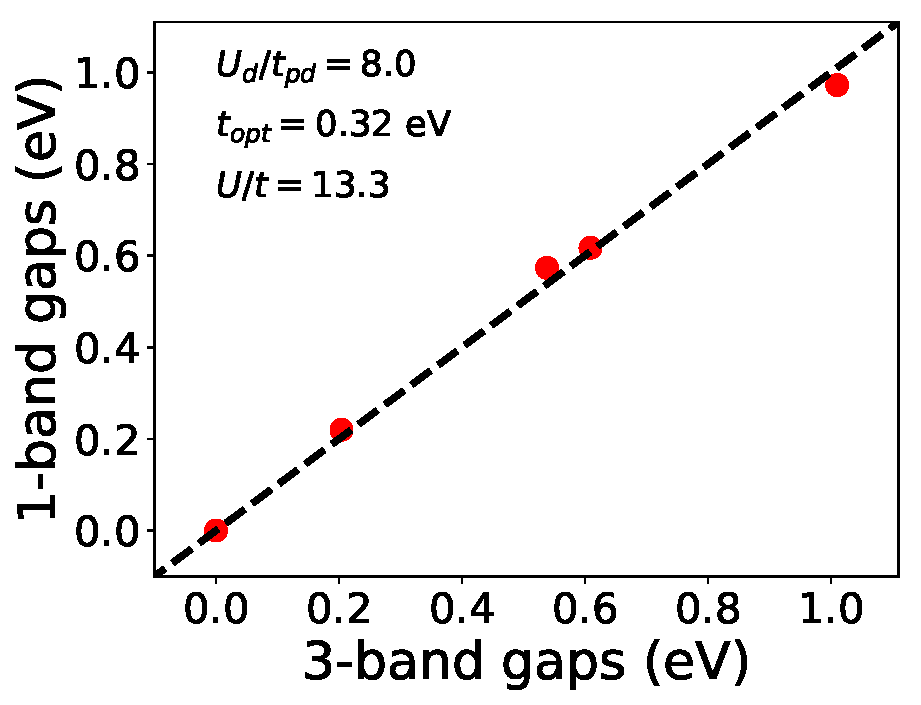
\includegraphics[width=0.325\linewidth]{./Figures/Gap_1_band_3_band_ep_3_number_9.pdf}
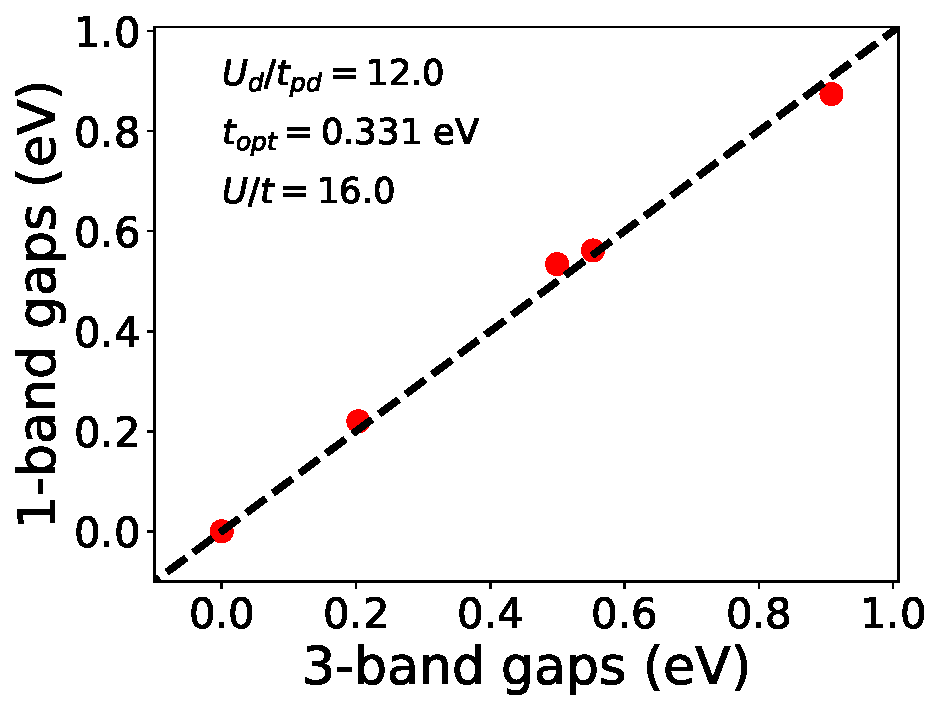
\includegraphics[width=0.325\linewidth]{./Figures/Gap_1_band_3_band_ep_3_number_2.pdf}
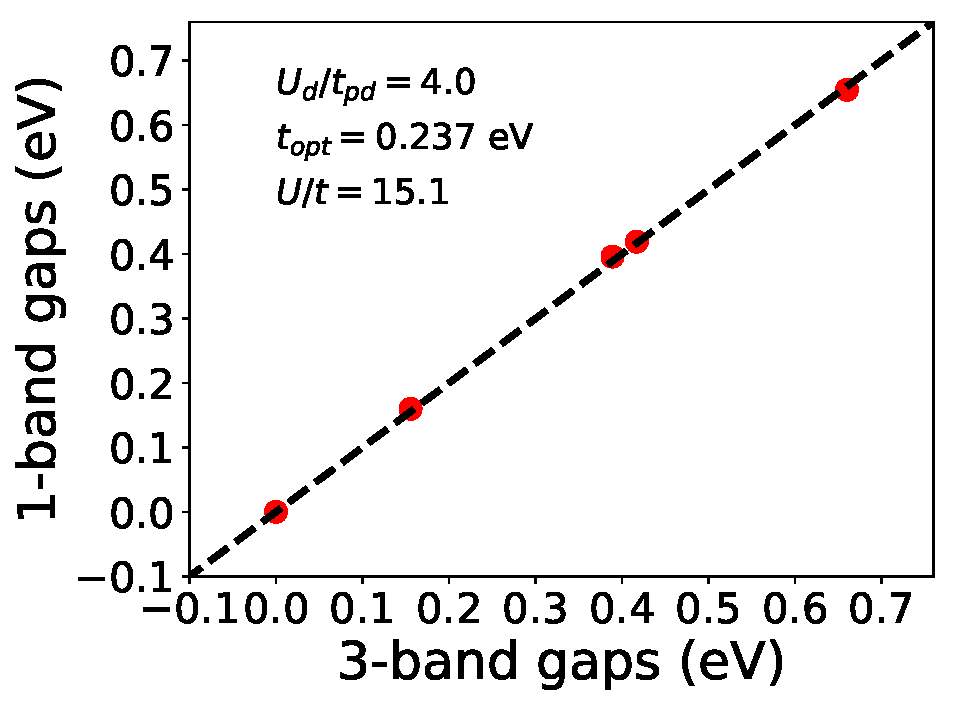
\includegraphics[width=0.325\linewidth]{./Figures/Gap_1_band_3_band_ep_5_number_5.pdf}
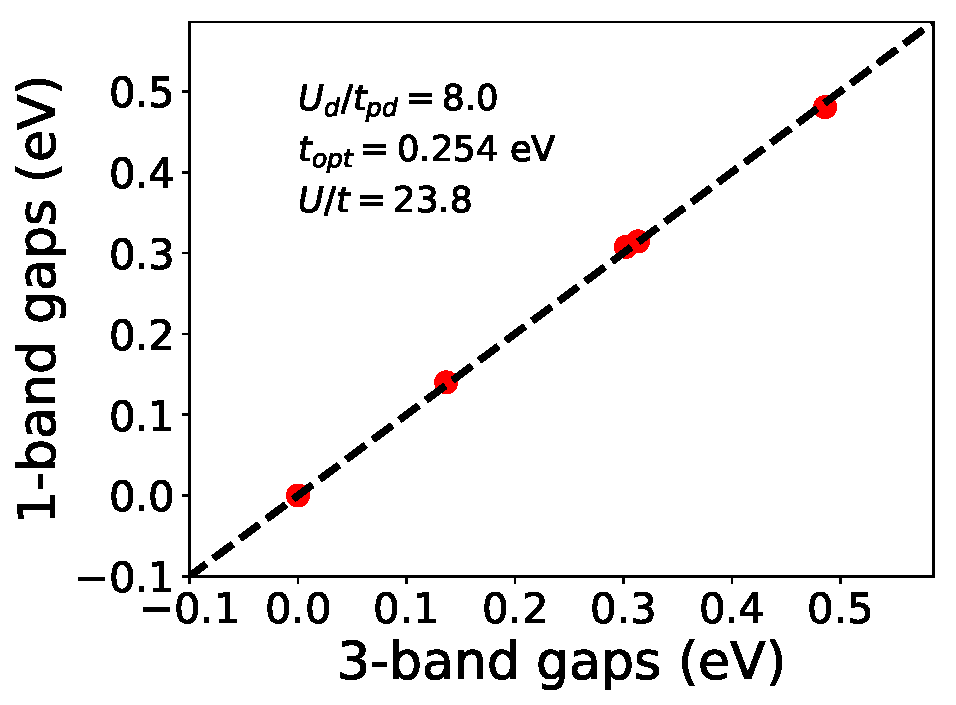
\includegraphics[width=0.325\linewidth]{./Figures/Gap_1_band_3_band_ep_5_number_9.pdf}
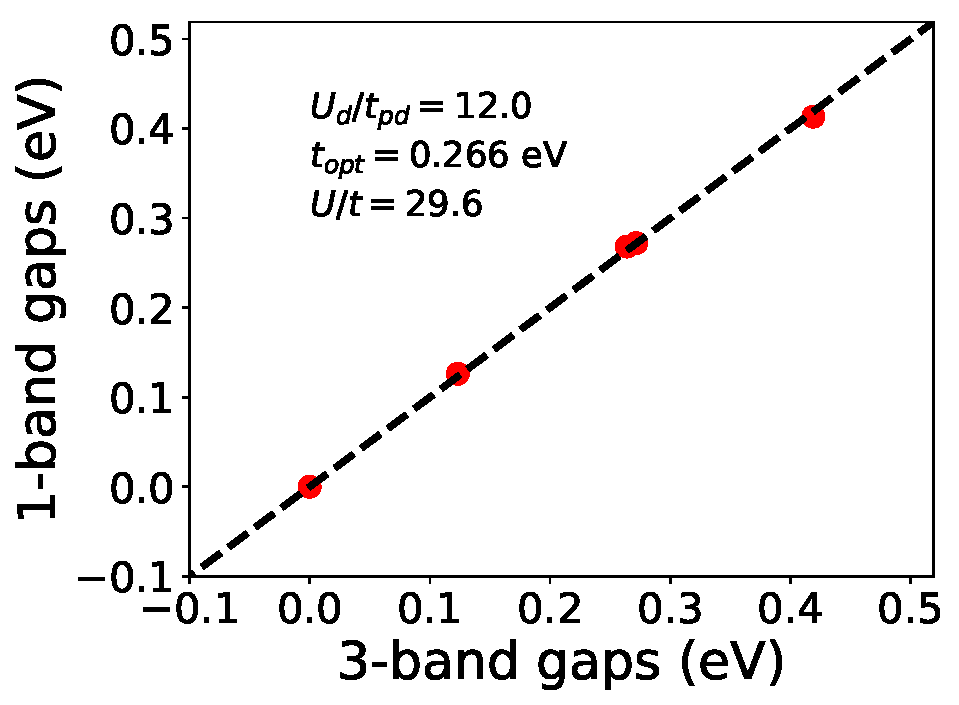
\includegraphics[width=0.325\linewidth]{./Figures/Gap_1_band_3_band_ep_5_number_2.pdf}
\caption{Comparison for energy gaps between the 3-band and 1-band Hubbard models using the optimized values of $U/t$ and $t$, for different
$U_{d}/t_{pd}$ for $\Delta/t_{pd}=3$ and $\Delta/t_{pd}=5$}
\label{fig:hamfit} 
\end{figure}	
Finally, we show that the obtained parameters are ....

